% it is essential to demonstrate that a proper professional approach was employed

% It should show how the project proposal was further refined and clarified, so that the implementation stage could go smoothly rather than by trial and error.

% You must demonstrate a structured design approach, including high-level design planning, design-for-test, consideration of human factors and systematic evaluation including confidence metrics within your evaluation where appropriate. You should explain how you would show conformance with appropriate legislation, such as that for intellectual property, data protection, human subjects and software licenses such as those for open source. Show that you understand the consequences of your project (or a more fully-formed variant of it) in terms of how it might affect commercial markets, contribute to society and/or the research community.

% Challenging and well-presented background covering Comp Sci topics beyond Part IB.

% Good requirements analysis, justified selection of suitable tools, good engineering approach.

\label{sec:2}

\section{Starting Point}
\label{sec:starting-point}
Visual SLAM systems are a mature and well-researched subfield of computer science with many advanced implementations. To avoid spending the majority of my effort re-implementing a visual SLAM system from scratch, I instead used a \textbf{single-agent} visual SLAM implementation as the starting point for my project. The rationale behind this decision was that it would allow me to focus my efforts on the distributed multi-agent aspect of this project, which I believe is the novel and under-researched aspect of the field.

I chose ORB-SLAM3 \autocite{ORBSLAM3_TRO} as the single agent SLAM system to base my system on top of, as it ranks at the top of benchmarks in a variety of environments \autocite{DBLP:journals/corr/abs-2108-01654} and its codebase is publically available. I primarily utilized the system's tracking and local mapping modules as well as some helper functions from the backend, which are all attributed during the discussion of my algorithms in the \nameref{sec:3} section.

While ORB-SLAM3 is an excellent SLAM system, it is fundamentally a single-agent system with no considerations in place for use in a multi-agent context. As I will later expand upon, a significant amount of time and effort was required to understand its extremely large undocumented codebase, especially since an almost complete understanding of its inner workings was needed to both extract and inject map information from the system. In retrospect, using an existing single-agent SLAM system as a foundation did not save as much time as it took almost a month to get ORB-SLAM compiled and running locally, and many more before I was able to make good progress on the distributed aspect of my project.

Nevertheless, using a cutting-edge single-agent SLAM system as a foundation for my project has allowed me to create a distributed SLAM system that performs better than comparable state-of-the-art systems, making it suitable for real-world applications.

At the time of submitting my project proposal, I had forked the ORB-SLAM3 git repository\footnote[1]{\url{https://github.com/UZ-SLAMLab/ORB_SLAM3}} and explored the codebase. ORB-SLAM3 is licensed under GPL-3.0, and as such, I have open-sourced my code under the same license.

I had no prior experience with SLAM systems but did research the current state of multi-agent visual SLAM systems to evaluate the feasibility of my project and to prevent it from being a duplication of prior work.


\section{Visual SLAM Background}
\label{sec:visual-slam-background}
Before developing a distributed multi-agent SLAM system, we must first understand the basics of a visual SLAM. This is a topic on which numerous books \autocite{gao2021introduction} \autocite{XiangGao} and research papers \autocite{durrant2006simultaneous} \autocite{taketomi2017visual} \autocite{10.1007} have discussed in depth, which I will attempt to summarize here. % This is a greatly simplified explanation, with modern SLAM implementations being tens of thousands of lines long.

\subsection{Visual Odometry}
\label{sec:visual-slam-visual-odometry}
To grasp visual SLAM effectively, it is useful to start with a foundational concept – visual odometry (VO). VO is the process of estimating the trajectory of a camera based on the sequence of images produced by it. The core idea is to track features across consecutive images, and by observing how the features move relative to one another it is possible to infer the motion of the camera.

Take, for example, the two images from the KITTI00 dataset \autocite{Geiger2013IJRR} presented in \autoref{fig:vo-example-images}. We can see that \autoref{fig:vo-example-image-b} is taken a few meters in front of \autoref{fig:vo-example-image-a} because the car on the left is closer in the second image, and the roof on the left becomes larger, et cetera. The goal of VO is to compute this change in pose between the two images.

\begin{figure}[h]
    \centering
    \begin{subfigure}[b]{0.475\textwidth}
        \centering
        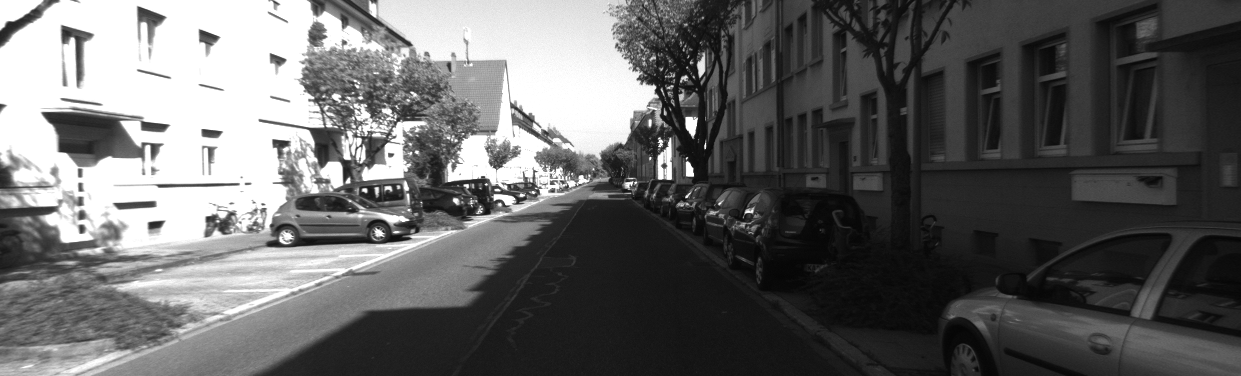
\includegraphics[width=\textwidth]{figures/vo_image_8.png}
        \caption{}
        \label{fig:vo-example-image-a}
    \end{subfigure}\hfill%
    ~
    \begin{subfigure}[b]{0.475\textwidth}
        \centering
        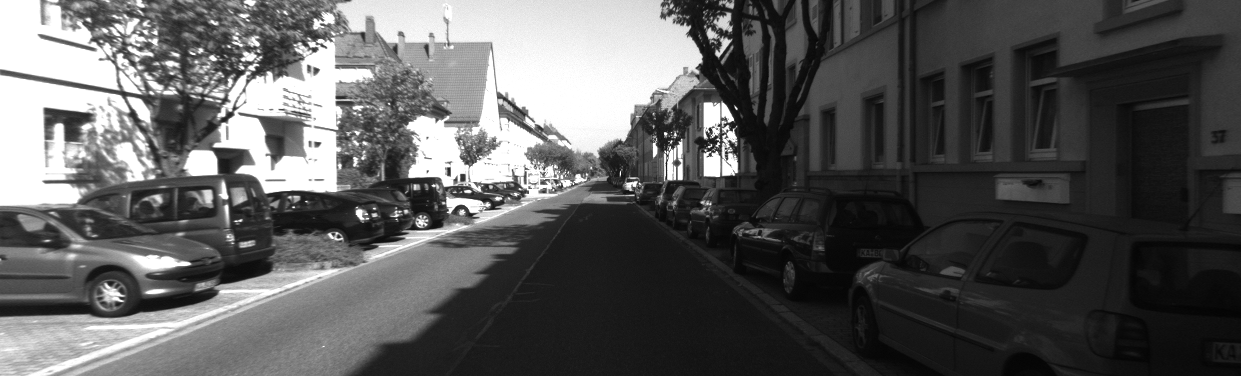
\includegraphics[width=\textwidth]{figures/vo_image_9.png}
        \caption{}
        \label{fig:vo-example-image-b}
    \end{subfigure}%
    \caption{Example images from KITTI00 dataset for visual odometry example.}
    \label{fig:vo-example-images}
\end{figure}

The first step towards determining the change in pose is identifying common features in both images. For this, we use feature descriptors, which find recognizable features within the image and represent them as a vector. A common feature descriptor used for VO and SLAM is the ORB descriptor \autocite{6126544}, due to its low computational cost and invariance to rotation and scale, and we will use it for this example.

\autoref{fig:vo-matches} displays the ORB feature matches between the two images, however it is clear that many of them are incorrect. This is to be expected, as many elements of the images are repeated (windows, trees, et cetera).

We can remove the majority of incorrect correlations by constraining the matches to the epipolar geometry model – essentially telling the computer that the two images are the same scene captured from two different camera poses. Since there are a lot of outliers we use the RANSAC algorithm, later defined in \autoref{sec:ransac}, to fit the data to the epipolar geometry model. This results in the matches identified in \autoref{fig:vo-matches-ransac}, which are far more accurate. We can see that the window on the left is correctly matched in the two images even though there are many similar windows in the images, demonstrating the importance of fitting our matches to the two-camera epipolar geometry model using RANSAC.

We can now run the seven-point algorithm \autocite{Hartley2004} on the matches to extract the rotation $\mathbf{R}$ and translation $\mathbf{t}$ between the two images, and consequently triangulate the world features found in both images. This is displayed in \autoref{fig:vo-3d-reconstruction}. By continuing this process for all image pairs in a video, we can estimate the trajectory of the camera as it moves through the world. It is important to note that the scale of the world is arbitrary when only using monocular video.

\begin{figure}[h]
    \centering
    \captionsetup{format=plain}
    \begin{minipage}[t]{0.475\textwidth}
        \centering
        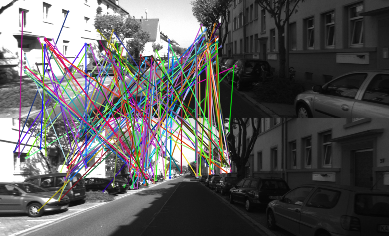
\includegraphics[width=\textwidth]{figures/vo_matches.pdf}
        \caption{Feature descriptor matches between the two images.}
        \label{fig:vo-matches}
    \end{minipage}\hfill%
    ~
    \begin{minipage}[t]{0.475\textwidth}
        \centering
        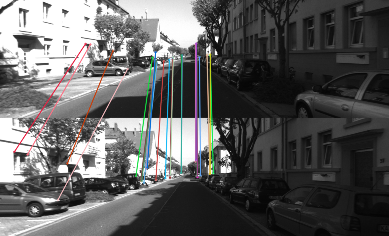
\includegraphics[width=\textwidth]{figures/vo_matches_ransac.pdf}
        \caption{Inlier feature descriptors after fitting the data to the epipolar geometry model using RANSAC.}
        \label{fig:vo-matches-ransac}
    \end{minipage}%
\end{figure}

\begin{figure}[h]
    \centering
    \begin{minipage}[t]{0.6\textwidth}
        \centering
        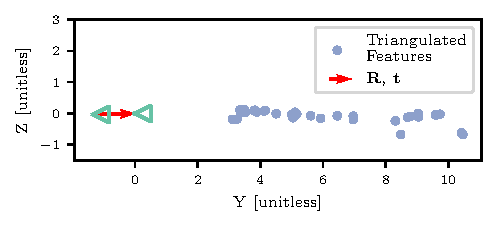
\includegraphics[width=\textwidth]{figures/3d_reconstruction.pdf}
        \caption{Side view of the estimated $\mathbf{R}$ and $\mathbf{t}$ between the two camera poses, and the triangulated feature points.}
        \label{fig:vo-3d-reconstruction}
    \end{minipage}%
\end{figure}

\subsection{Towards Visual SLAM}
\label{sec:towards-visual-slam}
Visual odometry provides a local estimate of trajectories, however, it does not build a map of the world and therefore can not give an accurate global estimate of the agent's trajectory. Visual SLAM solves this problem by constructing a map of the environment as it moves through it, using the map to localize itself within the world. Modern systems break this down into three processes: Tracking, Mapping, and Loop Closing.

\subsection{Tracking}
\label{sec:visual-slam-tracking}
The tracking step processes image data to compute the pose of the agent within the map. This step leverages many of the core ideas from visual odometry, using feature descriptors to find matches and fitting them to the epipolar geometry model using RANSAC. However, instead of matching features between consecutive images like visual odometry, we find feature matches between the input image and the map we have built. This is possible because the map is essentially a set of feature descriptors and their estimated position in 3D space, allowing our tracking module to find matches and localize the agent.

\subsection{Mapping}
\label{sec:visual-slam-mapping}
Mapping extracts the data gathered during the tracking phase to create a 3D representation of the environment. Many popular visual SLAM implementations use a keyframe-based approach, where the map is estimated using only a few select image frames, ignoring the intermediate frames which provide little new information. This effectively decouples the mapping and tracking processes, allowing us to perform relatively costly but very effective pose graph optimizations.

\textbf{Pose Graph Optimization} is the process of minimizing the errors within our map, typically through the use of a graph optimizer. We represent keyframes and world features as nodes in our graph, with edges representing the constraints between nodes through a cost function. For example, if a keyframe observes a feature at position (-0.23, 0.64) in their image, an edge between the keyframe and feature will be created with a cost function that is minimized when the feature is re-projected onto the keyframe at the observed point. Similar edge constraints can be defined between keyframes using IMU measurements or wheel odometry. A graph optimizer can then be used to tweak the keyframe poses and feature locations to minimize the cost functions, therefore improving our map's accuracy.

We can intuitively think of the edge constraints as springs (\autoref{fig:gpo-diagram}), all attempting to revert to their preferred length (given by the world observations). The graph optimizer moves the keyframes and features around until the system settles into its lowest energy state, where the map agrees with our observations as closely as possible.

\begin{figure}[h]
    \centering
    \begin{minipage}[t]{0.6\textwidth}
        \centering
        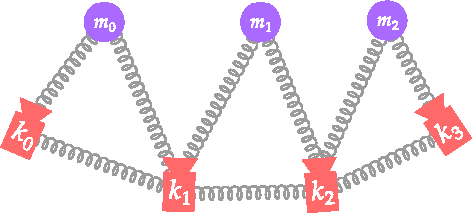
\includegraphics[height=1.4in]{figures/gpo_diagram.pdf}
        \caption{Graph pose optimization diagram, where $k_i$ is a keyframe and $m_i$ is a feature point. The springs represent constraints between the nodes.}
        \label{fig:gpo-diagram}
    \end{minipage}%
\end{figure}

\subsection{Loop Closure}
\label{sec:visual-slam-loop-closure}
Loop closing is crucial for maintaining the long-term accuracy of the SLAM system. It involves recognizing when the agent re-visits a previously mapped location and ``closes the loop'' by correcting the errors that have accumulated over time. We often vectorize keyframes using the visual bag of words approach (later explained in \autoref{sec:visual-bag-of-words}) to identify when an agent re-visits an area. When a loop closure is detected, we fuse the duplicate features and use pose graph optimization to re-optimize the map and ensure global consistency, as illustrated in \autoref{fig:gpo-loop-closure}.

\begin{figure}[h]
    \centering
    \begin{subfigure}[t]{0.54\textwidth}
        \centering
        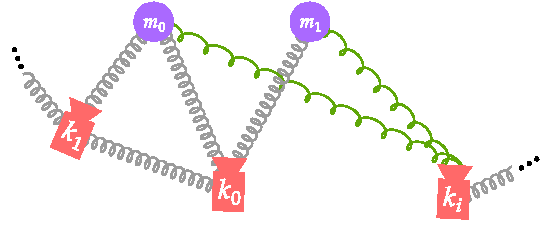
\includegraphics[width=\textwidth]{figures/gpo_loop_closure_1.pdf}
        \caption{A loop closure is identified and new constraints are added between $k_i$ and $m_0$, $m_1$. The new constraints are initially ``stretched'' since $m_0$ and $m_1$'s location in the map does not correlate with $k_i$'s observation of them.}
    \end{subfigure}\hfill%
    ~
    \begin{subfigure}[t]{0.43\textwidth}
        \centering
        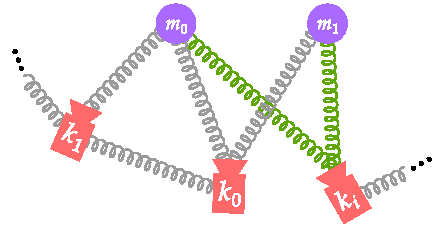
\includegraphics[width=\textwidth]{figures/gpo_loop_closure_2.pdf}
        \caption{The graph optimizer adjusts the keyframes and feature point poses so the map better aligns with the observations.}
    \end{subfigure}%
    \caption{Loop closure pose graph optimization. The green edges represent the new constraints added by the loop closure.}
    \label{fig:gpo-loop-closure}
\end{figure}


\section{Relevant Work}
\label{sec:relevant-work}
While single-agent SLAM systems are a relatively mature field of research, multi-agent systems are still very much in active development.

Centralized multi-agent systems such as CCM-SLAM \autocite{schmuck2019ccm} and COVINS \autocite{schmuck2021covins} require a centralized server to perform map merges and PGO. While simpler to implement, this comes with the obvious limitations of centralized systems such as scalability issues and requiring existing networking infrastructure.

In recent years we have seen the emergence of a handful of decentralized multi-agent systems, however, many have various limitations. Systems such as \autocite{doi:10.1126/scirobotics.abm5954} \autocite{8658783} \autocite{DBLP:journals/corr/abs-2103-12770} require the agents to be initialized with their ground truth poses, which greatly limits their real-world usability. In contrast, my system is able to provide accurate relative localization even when agents are initialized in arbitrary and unknown locations by identifying common landmarks in the world.

\autoref{fig:related-work-sensor-configurations} lays out the sensor configurations used by popular state-of-the-art multi-agent SLAM systems, showing that my system is one of the only distributed systems capable of operating with purely monocular visual data\footnote[1]{There are several other monocular-only systems published in the field \autocite{egodagamage2017collaborative} \autocite{chen2018distributed} \autocite{bresson2012real}. However, unlike most other systems, they have not made their source code available, nor have they reported their system performance on publicly accessible datasets. Unfortunately, this makes any meaningful comparisons to their systems impossible.}. This is advantageous, as LiDAR \& RGBD sensors have considerable weight, and stereo cameras may require a minimum camera separation to operate, both of which limit their usage on small aerial robots. However, using only monocular video introduces several challenges, such as less data being available to perform tracking and mapping, and agents' maps having an arbitrary scale.

\begin{figure}[h]
    \centering
    \adjustbox{valign=t, width=\linewidth}{
        \def\arraystretch{1.2}
        \begin{tabular}{ |l|c|c|c|c|c|c|c|c| }
            \hline
            \multirow{2}{*}{\textbf{System}}                       & \multirow{2}{*}{\textbf{Year}} & \textbf{Collaboration} & \multirow{2}{*}{\textbf{Monocular}} & \multirow{2}{*}{\textbf{Stereo}} & \textbf{Monocular}     & \textbf{Stereo}        & \textbf{LiDAR}         & \textbf{RGBD}          \\
                                                                   &                                & \textbf{Type}          &                                     &                                  & \textbf{\texttt{+}IMU} & \textbf{\texttt{+}IMU} & \textbf{\texttt{+}IMU} & \textbf{\texttt{+}IMU} \\

            \hline
            \textbf{My System}                                     & 2024                           & Decentralized          & X                                   &                                  &                        &                        &                        &                        \\
            \hline
            \textbf{$D^2$SLAM \autocite{xu2022d}}                  & 2022                           & Decentralized          &                                     &                                  &                        & X                      &                        &                        \\
            \hline
            \textbf{CCM-SLAM \autocite{schmuck2019ccm}}            & 2019                           & Centralized            & X                                   &                                  &                        &                        &                        &                        \\
            \hline
            \textbf{COVINS \autocite{schmuck2021covins}}           & 2021                           & Centralized            &                                     &                                  & X                      &                        &                        &                        \\
            \hline
            \textbf{Kimera-multi \autocite{tian22tro_kimeramulti}} & 2021                           & Decentralized          &                                     &                                  &                        & X                      &                        & X                      \\
            \hline
            \textbf{Swarm-SLAM \autocite{lajoieSwarmSLAM}}         & 2024                           & Decentralized          &                                     &                                  &                        & X                      & X                      & X                      \\
            \hline
            \textbf{DOOR-SLAM \autocite{Lajoie2020DOORSLAM}}       & 2020                           & Decentralized          &                                     &                                  &                        & X                      &                        &                        \\
            \hline
        \end{tabular}
    }

    \caption{Comparison of popular multi-agent SLAM systems. My SLAM system stands out as one of the only modern decentralized monocular systems available\protect\footnotemark[1].}
    \label{fig:related-work-sensor-configurations}
\end{figure}

Additionally, my system provides a novel approach to the Distributed Pose Graph Optimization (DPGO) problem. There are various approaches to DPGO. SWARM-SLAM \autocite{Lajoie_2024} elects a single agent to perform the PGO for the entire swarm, which is simple but has a high communication overhead since all agents have to send their pose estimations before each optimization. Other systems perform DPGO by spreading computation across agents by using algorithms such as ARock \autocite{Peng_2016} or Distributed Gauss-Seidel \autocite{DBLP:journals/corr/ChoudharyCNRCD17}, however these methods still present a communication overhead and may stall in when presented with unreliable communications.

Instead of performing discrete optimization runs, my method of DPGO is performed incrementally. Each agent optimizes its pose graph as external data streams in, with a separate map alignment step. This method has no additional communication overhead, apart from the infrequent map alignment step, however, it comes at the cost of less verifiable global consistency. We evaluate my method's performance in the \nameref{sec:benchmarking} section, demonstrating its very competitive real-world performance. The details of my implementation are presented in the \nameref{sec:decentralized-system-manager} section.


% DOOR-SLAM(2020) \autocite{Lajoie2020DOORSLAM} uses the Distributed Gauss-Seidel approach to Distributed Pose Graph Optimization (DPGO) proposed by Choudhary et al. in 2017 \autocite{DBLP:journals/corr/ChoudharyCNRCD17} while Kimera-Multi(2022) \autocite{tian22tro_kimeramulti} utilizes distributed graduated non-convexity for DPGO. However,

% Xu et al. \autocite{xu2022d} argue that DOOR-SLAM(2020) \autocite{Lajoie2020DOORSLAM} and Kimera-Multi(2022)'s distributed pose graph optimization methods prevent their systems from achieving accurate relative localization. $D^2$SLAM(2022)'s \autocite{xu2022d} near field and far field estimation systems allow it to achieve accurate relative localization while maintaining global consistency, however it

% often use some method of distributed optimization to refine the shared map. Most commonly this is done using Distributed Pose Graph Optimization (DPGO), which globally optimizes the shared map, providing good global consistency but often lacking in relative localization

% Distributed Pose Graph Optimization (DPGO) is the most common technique used in multi-agent SLAM systems. DPGO represents

% $D^2$SLAM(2022) \autocite{xu2022d} uses pose graph  (PGO)



% While traditionally under-researched, there have been a multi-agent SLAM systems that have recently

% Single-agent visual SLAM is a very well-researched field, with many advanced implementations available, such as VINS-Mono(2018) \autocite{8421746}, Kimera(2019) \autocite{rosinol2020kimera} and ORB-SLAM3(2020) \autocite{ORBSLAM3_TRO}.

% While single-agent systems are very mature at this point, C-SLAM is a developing field with exciting advancements being made in recent years. C-SLAM is split into two categories: centralized and decentralized. Centralized C-SLAM systems require a centralized server to manage communication between agents and perform map merging. Some examples include CCM-SLAM(2019) \autocite{schmuck2019ccm} and COVINS(2021) \autocite{schmuck2021covins}.

% We will primarily focus on decentralized C-SLAM systems

% todo: add comparison table?

\section{Algorithms}
\label{sec:algorithms}
This section will briefly cover some of the existing algorithms utilized within my SLAM system and can be used as a reference when reading the \nameref{sec:3} section.

\subsection{Kabsch-Umeyama Algorithm}
\label{sec:kabsch-umeyama-algorithm}
The Kabsch-Umeyama algorithm (\autoref{alg:kabsch-umeyama}) is used to align a set of target points $Q$ to a set of source points $P$ with a SIM(3) transform. Within the field of SLAM, this is primarily used to align the estimated trajectory with the ground truth, as it may be translated, rotated, and scaled differently to the ground truth. Additionally, this algorithm is used for my multi-agent map alignment process.

\begin{algorithm}[H]
    \setstretch{1.2}
    \caption{Kabsch-Umeyama Algorithm}
    \label{alg:kabsch-umeyama}
    \begin{algorithmic}[1]
        \State \textbf{Input:} Source points $P$, target points $Q$
        \State \textbf{Output:} Rotation $R$, scale $s$, and translation $t$ that best aligns $Q$ to $P$
        \State $n \gets \text{number of points in each set}$
        \State $\mu_P \gets \frac{1}{n} \sum_{i=1}^n p_i$
        \State $\mu_Q \gets \frac{1}{n} \sum_{i=1}^n q_i$
        \State $P' \gets P - \mu_P$ \Comment{Centering $P$}
        \State $Q' \gets Q - \mu_Q$ \Comment{Centering $Q$}
        \State $\sigma^2_P \gets \frac{1}{n} \sum_{i=1}^n ||p_i'||^2$ \Comment{Variance of P}
        \State $H \gets \frac{1}{n} \sum_{i=1}^n p_i'^T q_i'$ \Comment{Covariance matrix}
        \State $U, D, V^T \gets \text{SVD}(H)$ \Comment{Singular Value Decomposition}
        \State $S \gets \text{diag}(1, 1, \dots, 1, \det(U)\det(V^T))$
        \State $R \gets USV^T$ \Comment{Rotation matrix}
        \State $c \gets \frac{\sigma^2_P}{\text{tr}(DS)}$ \Comment{Scale factor}
        \State $t \gets \mu_P - cR\mu_Q$ \Comment{Translation}
        \State \textbf{return} $R, s, t$
    \end{algorithmic}
\end{algorithm}

\subsection{Visual Bag of Words}
\label{sec:visual-bag-of-words}
Visual bag of words representation is used to vectorize an image based on its features, allowing us to compare how similar two images are. My system utilizes this to efficiently detect potential map merges between agents.

To convert our image to a vector, we must first build a \textit{vocabulary} of features – common and unique features that will each go on to represent a dimension of our image vector. We do this by first extracting features from a large dataset of images and grouping their descriptors using an algorithm such as K-Means clustering. The center of the largest clusters can then be used as our feature vocabulary. A visual overview of the process is given in \autoref{fig:bow-vocab}. This vocabulary generation step only needs to be performed once, preferably using a wide variety of representative images (for visual SLAM this could be images from a variety of environments).

We are now able to vectorize images by counting the number of times each feature within our vocabulary exists in the image (\autoref{fig:bow-vector}).

\begin{figure}[h]
    \captionsetup{format=plain}
    \begin{minipage}[t]{0.55\linewidth}
        \centering
        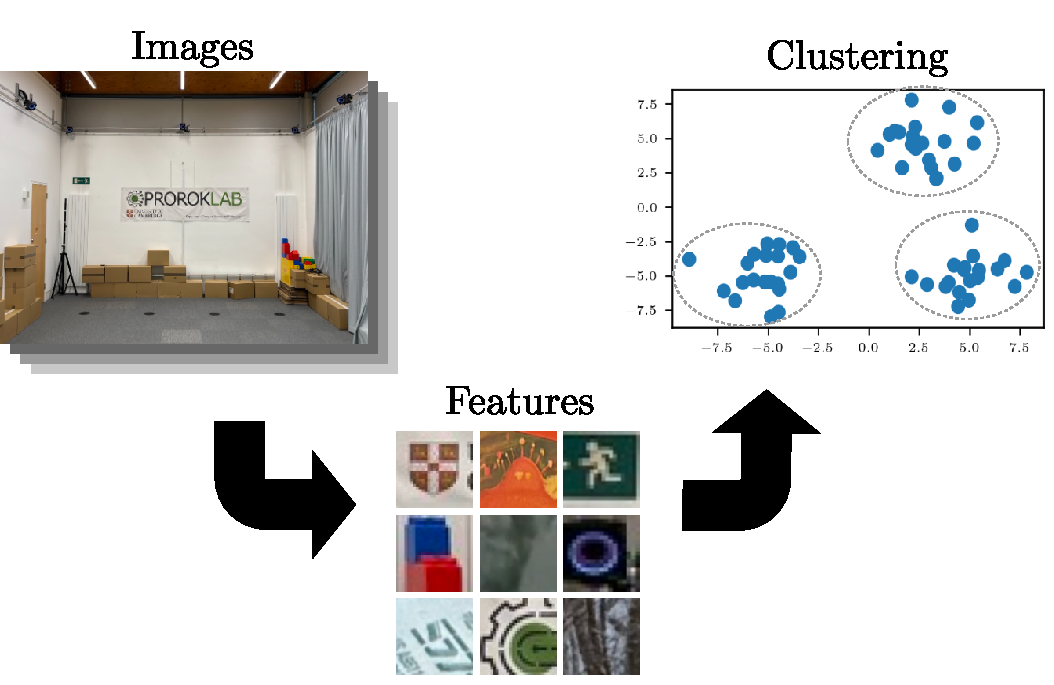
\includegraphics[width=\linewidth]{figures/bow_vocab.pdf}

        \caption{Process of generating the visual bag of word vocabulary. The center of each cluster is added as a feature in the vocabulary and represent a distinct vector dimension.}
        \label{fig:bow-vocab}
    \end{minipage}\hfill%
    ~
    \begin{minipage}[t]{0.4\linewidth}
        \centering
        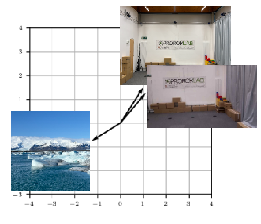
\includegraphics[width=\linewidth]{figures/bow.pdf}
        \caption{Visualization of image vectorization using the visual bag of words method. Images sharing common features result in closely aligned vectors.}
        \label{fig:bow-vector}
    \end{minipage}
\end{figure}

\subsection{RANSAC}
\label{sec:ransac}

RANdom SAmple Consensus (RANSAC) is an iterative method used to robustly fit a mathematical model to a dataset with a large number of outliers, with the outliers having no influence over the estimated model. This is particularly useful in visual SLAM as observations are extremely noisy, often containing far more outliers than inliers. Pseudocode for the algorithm is presented in \autoref{alg:ransac}.

\begin{algorithm}[h]
    \caption{RANSAC Algorithm}
    \label{alg:ransac}
    \begin{algorithmic}[1]
        \State \textbf{Input:} dataPoints, model to explain data, number of iterations $k$, threshold $\tau$, minimum number of data points needed to fit model $n$
        \State \textbf{Output:} Best fitting model

        \State bestmodel $\leftarrow$ null
        \State bestInliers $\leftarrow$ \{\}

        \For{$i = 1$ to $k$}
        \State samples $\leftarrow$ $n$ randomly selected data points
        \State model $\leftarrow$ model fit to samples
        \State inliers $\leftarrow$ \{\}

        \For{each point in dataPoints}
        \If{point fits model with error $<$ $\tau$}
        \State Add point to inliers
        \EndIf
        \EndFor

        \If{number of inliers $>$ size of bestInliers}
        \State bestInliers $\leftarrow$ inliers
        \State bestModel $\leftarrow$ model
        \EndIf
        \EndFor

        \State \Return bestModel
    \end{algorithmic}
\end{algorithm}

\section{Requirements Analysis}
\label{sec:requirements-analysis}
After further background reading on the subject and a review of other multi-agent SLAM systems, I broke my project down into the requirements shown in \autoref{fig:risk-analysis}. Features vital to achieving my core deliverables are given high importance, while extensions are given low importance. Additionally, features are given a risk level depending on how research-heavy they were, which helped me when planning and allocating time.


\begin{figure}[h]
    \centering
    \captionsetup{justification=raggedright,singlelinecheck=false,margin={1in,1in}}
    \adjustbox{valign=t, width=4in}{
        \def\arraystretch{1.2}

        \newcommand{\highentry}[0]{
            \colorbox{Red!40!White}{\texttt{ High \vphantom{|g}}}
        }
        \newcommand{\mediumentry}[0]{
            \colorbox{Yellow!50!White}{\texttt{Medium\vphantom{|g}}}
        }
        \newcommand{\lowentry}[0]{
            \colorbox{Green!40!White}{\texttt{\: Low \:\vphantom{|g}}}
        }


        \begin{tabular}{ lcc }
            \hline
            \textbf{Feature}                    & \textbf{Importance} & \textbf{Risk} \\
            \hline
            Simulation environment              & \highentry          & \lowentry     \\
            ORB-SLAM3 integration               & \highentry          & \mediumentry  \\
            Map serialization/deserialization   & \highentry          & \mediumentry  \\
            Decentralized system state manager  & \highentry          & \lowentry     \\
            Map merge finder and merger         & \highentry          & \lowentry     \\
            Handle losing communication         & \highentry          & \lowentry     \\
            Management interface                & \mediumentry        & \lowentry     \\
            Distributed pose graph optimization & \lowentry           & \highentry    \\
            Map compression                     & \lowentry           & \mediumentry  \\
            Visualization tools                 & \lowentry           & \lowentry     \\
            Additional sensors                  & \lowentry           & \highentry    \\
            Intelligent map sharing             & \lowentry           & \mediumentry  \\
            Motion controller$^1$               & \lowentry           & \mediumentry  \\
            Real-world deployment$^1$           & \lowentry           & \mediumentry  \\
            Augmented Reality visualization$^1$ & \lowentry           & \highentry    \\
        \end{tabular}
    }

    \caption{Risk analysis.\captionbreak$^1$Requirements added after work had begun.}
    \label{fig:risk-analysis}
\end{figure}

\subsection{Development Model}
\label{sec:development-model}
This project lends itself best to the Spiral Development Model \autocite{59}, as it consists of multiple well-defined features but requires frequent review and planning to decide what direction to push the project forward next. Developing my SLAM system was a large software engineering undertaking, involving the development of 5 ROS packages, an evaluation library, and even hardware. I knew that a rigid plan would quickly fall apart as roadblocks occurred, and therefore, I chose the spiral model as it allowed me to adapt my plan as risks were identified and priorities were changed.

After implementing each core feature of my SLAM system, I would evaluate its performance with my testing and evaluation infrastructure to identify any unexpected issues and identify potential risks. This would influence my plan for the next iteration around the spiral, as well as my long-term plan for the project.

A good example of a pivot taken after re-evaluating my project was in late January, when the core features of my project were complete and I was planning the next stage of development. Discussions with my supervisor, as well as my own analysis of the project, revealed that the original extensions were no longer very relevant to my project, as they either had implicitly been achieved while developing my core features or would not yield particularly interesting results. We instead decided to focus on deploying to real robots to demonstrate real-world usability and performance. I am glad that I made this choice, as I believe it greatly strengthens the credibility of my SLAM system.

\subsection{Licensing}
\label{sec:licensing}
All my code is available as open-source software on GitHub. The core SLAM system and Multi-Agent EVO library are released under the GPL-3 license \autocite{gplv3} as it builds upon code released under that license. My Raspberry Pi Video Publisher is published under the MIT license \autocite{mit}.

\section{Development Tools \& Frameworks}
\label{sec:development-tools-and-frameworks}
Due to this project being a large software engineering undertaking, I knew that a well-structured development plan and carefully chosen frameworks would be essential to the successful implementation of this project. Much thought was put into using frameworks such as ROS and Docker, all of which allowed my system to easily be deployed to real-world robots.

In addition, an entire suite of infrastructure had to be developed to aid the development of my distributed SLAM system, including simulation environments, an evaluation library, and testing infrastructure.

\subsection{Webots Simulation Software}
\label{sec:webots-simulator}

Robotics projects work in the physical domain, however testing in the real world requires a large amount of setup and infrastructure. To ensure fast iteration, I decided to use simulations for the majority of my development. This allowed me to easily test my system in various environments and scenarios before deploying it to physical robots.

The details of integrating Webots into my project are explored in the \autoref{sec:simulation-environment} section, including the ROS interfaces developed and agent controllers.

\subsection{Testing Infrastructure}
\label{sec:testing-infrastructure}

Along with being very useful for real-time testing, the simulation software enabled me to record numerous test cases which I have used as regression tests and benchmarks for my system throughout development.

I have built a central management interface that allows me to record and replay datasets from the simulation software, among many other functions. There are datasets for testing all core functionality of my SLAM system, which I would run at regular intervals during development to ensure that no features had regressed and to ensure performance was improving. The central management interface's implementation is further explained in \autoref{sec:central-management-interface}.

\subsection{Robot Operating System 2 Communication Middleware}
\label{sec:ros-2}
Robot Operating System (ROS) 2 is the glue holding my system together, allowing independent software processes and hardware to communicate through an abstract messaging interface.

ROS has long been the industry standard, being almost ubiquitous in both robotics research and the commercial sector. Confusingly, ROS is not an operating system at all, but instead, a cross-platform development framework that provides a middleware to facilitate reliable communication between independent processes called \textit{nodes}. These nodes can be on the same device or a device within the local area network and may be written in C++ or Python. Nodes communicate by \textit{publishing} and \textit{subscribing} to different \textit{topics}, allowing both peer-to-peer communication and broadcasting.

% This is best illustrated with an example. Below is a toy-distributed SLAM system. Given agents $\{ \texttt{agent}_n \ | \ n \in \{1, 2\} \}$, each agent has a camera which publishes to the $\texttt{/agent}_n$\verb|/camera| topic. The $\texttt{SLAM\_Processor}_n$ node subscribes to the $\texttt{/agent}_n$\verb|/camera| topic, and performs simultaneous localization and mapping using the image stream. The $\texttt{SLAM\_Processor}_n$ node then publishes to the $\texttt{/agent}_n$\verb|/new_map_data| topic, which the other agent can subscribe to and use to improve their local map.

% todo: add diagram

Since every node is abstracted away behind the interface provided by the various messaging topics, we can easily swap out nodes in this system. For example, we can substitute the real camera for a simulated camera to test my system in a virtual environment without having to change any other part of the system – as shown in \autoref{fig:abstract-camera-interface}. This makes transitioning between the real and simulated world almost seamless, which I knew would be essential for the eventual deployment on to physical robots.

\begin{figure}[h]
    \centering
    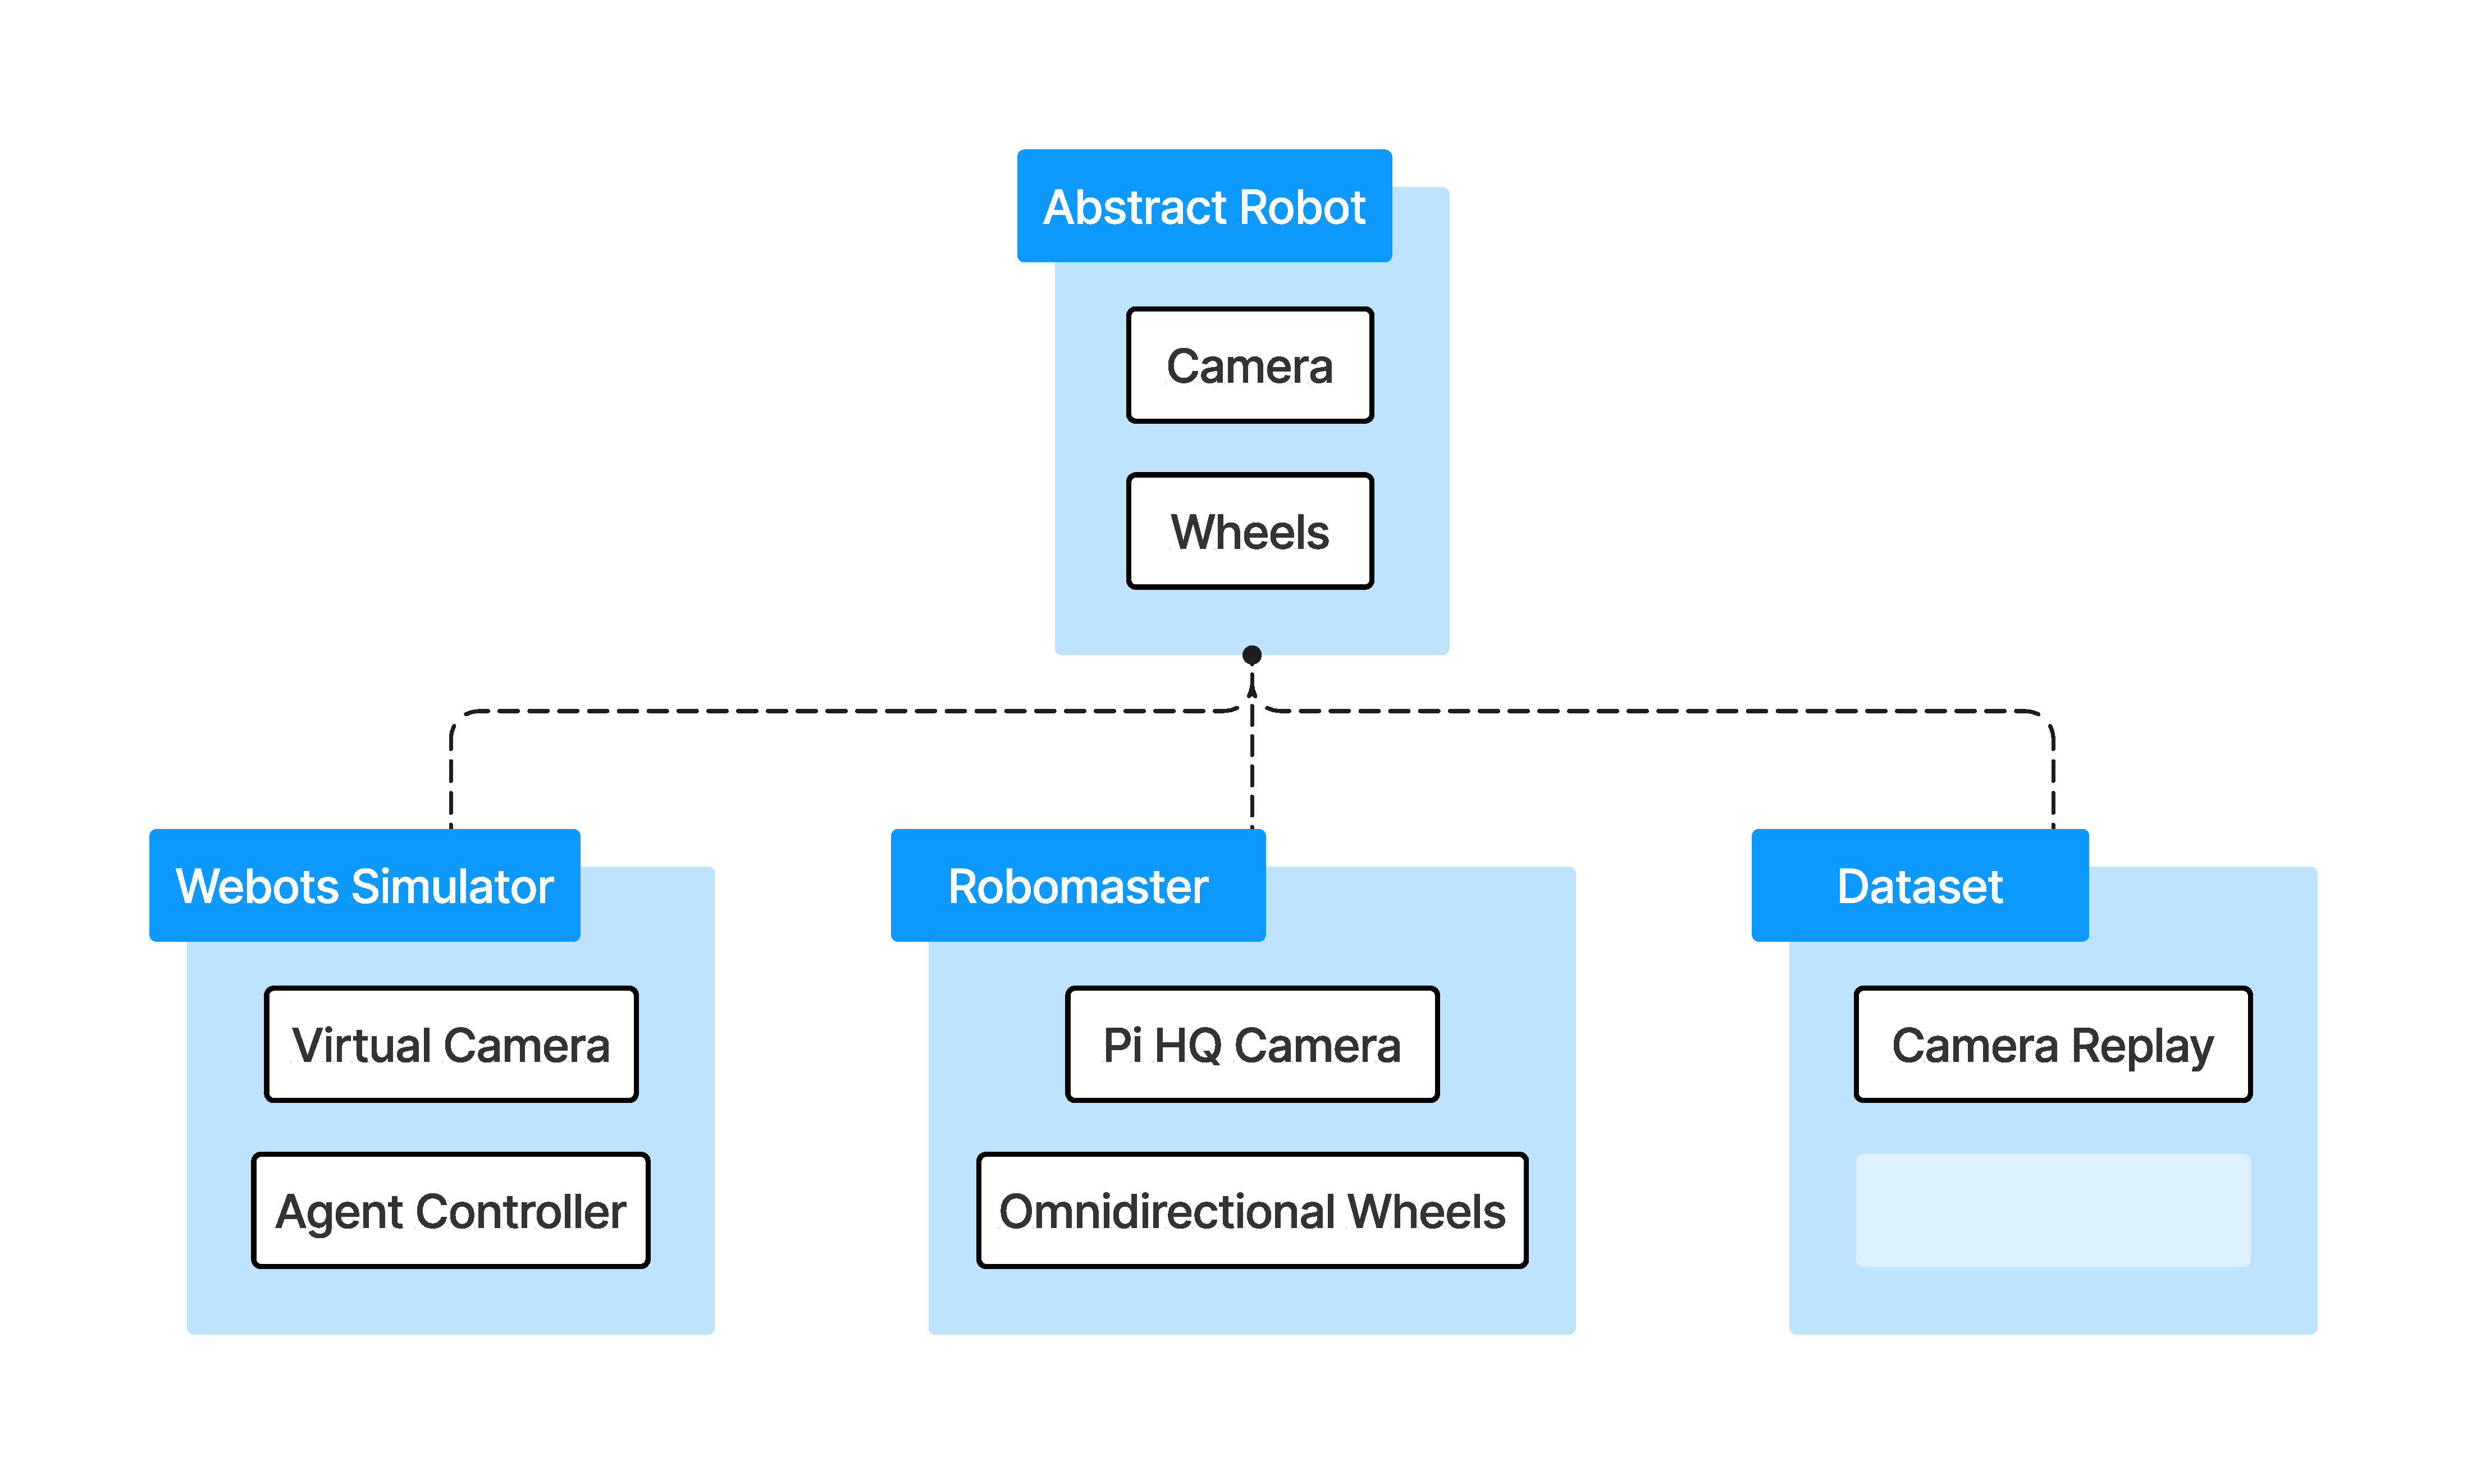
\includegraphics[trim=5cm 5cm 5cm 5cm, scale=0.15]{figures/abstract_camera_interface.pdf}

    \caption{All robot types inherit the abstract robot interface as they all use the same ROS message types. This allows my SLAM system and its supporting infrastructure to be completely agnostic to the actual type of robot used.}
    \label{fig:abstract-camera-interface}
\end{figure}

Furthermore, using the ROS framework allows my code to be far more portable, as anyone can download my nodes, link the camera topics up to their robot's camera, and run my SLAM system with minimal effort. This allows my system to be easily reproducible and not tied to particular hardware.

There are two versions of ROS: ROS 1 and ROS 2. I chose to use ROS 2 due to its improved decentralized properties, which align with the goals of this project. ROS 2 conforms to the Data Distribution Service (DDS)\footnote[1]{\url{https://en.wikipedia.org/wiki/Data_Distribution_Service}} specification, which guarantees a reliable broadcast and, unlike ROS 1, it does not require a leader node when used in a multi-agent setup.

\subsection{Repository Setup}
\label{sec:repository-setup}
It was essential for me to set up my repository properly before beginning work on this project. Since the majority of my initial effort was spent understanding and modifying ORB-SLAM3, I set up clangd to add smart code suggestions to my project based on my CMake profile. This was extremely helpful, as ORB-SLAM3 had no documentation or comments, and variables were often not given useful names. Additionally, I set up formatters to autoformat my C++ and Python code on save.

Throughout my project, I made extensive use of the GNU Project Debugger to identify bugs within my codebase, especially issues brought about by multithreading.

The five ROS packages in my repository also follow the standard ROS file structure, allowing others to easily understand and modify them.

\subsection{Docker Containers}
\label{sec:docker-containers}
Docker containers are used on all physical deployments of my software, including the Cambridge RoboMasters used for real-world testing of my SLAM system and my Raspberry Pi Video Publisher platform which is used for custom dataset collection and augmented reality visualizations.

Docker allows the software to be isolated in self-sufficient environments, making it easy to deploy on different computing environments. Additionally, using Docker allows my code to be built once and then deployed on multiple robots, preventing the need to rebuild the system on every robot which saves a significant amount of time. These aspects of Docker are expanded upon in the section below.

\subsection{Continuous Integration / Continuous Deployment}
\label{sec:cicd}
My GitHub repositories are set up to perform continuous integration via GitHub Actions. Every time code is pushed to the repository, all 5 core packages (\texttt{controller}, \texttt{interfaces}, \texttt{motion\_controller}, \texttt{orb\_slam3\_ros}, \texttt{webots\_sim}) are built to ensure there are no compile time errors.

Additionally, a Docker container is cross-compiled to \texttt{arm64} and uploaded to Docker Hub. These Docker images can then be downloaded to the Cambridge RoboMasters (the platform used for real-world testing) and immediately run. The pipeline is illustrated in \autoref{fig:cicd-diagram}. This greatly speeds up development, as compiling the codebase locally on the Cambridge RoboMasters takes over 20 minutes for each robot.

Aside from the core packages, we also perform continuous integration as well as continuous deployment for the Raspberry Pi video publisher package, later introduced in \autoref{sec:raspberry-pi-video-publisher}. A Docker container is similarly cross-compiled to \texttt{arm64} and uploaded to Docker Hub, and it is automatically deployed to the Raspberry Pis so they will run the latest version of the package.

Continuous deployment makes sense for this use case as the Raspberry Pis are designed to be plug-and-play, starting video streaming as soon as they are turned on. Unlike the Cambridge RoboMasters which are frequently ssh'ed into to pull specific Docker images and start experiments, we want the Raspberry Pis to use the latest software as soon as it is pushed to the GitHub repository.

The ease of use of the Raspberry Pi ROS video publisher platform that I have developed has made them an invaluable tool and resolves the time-syncing issues previously faced when using the existing cameras in the Prorok Lab.

\begin{figure}[h]
    \centering
    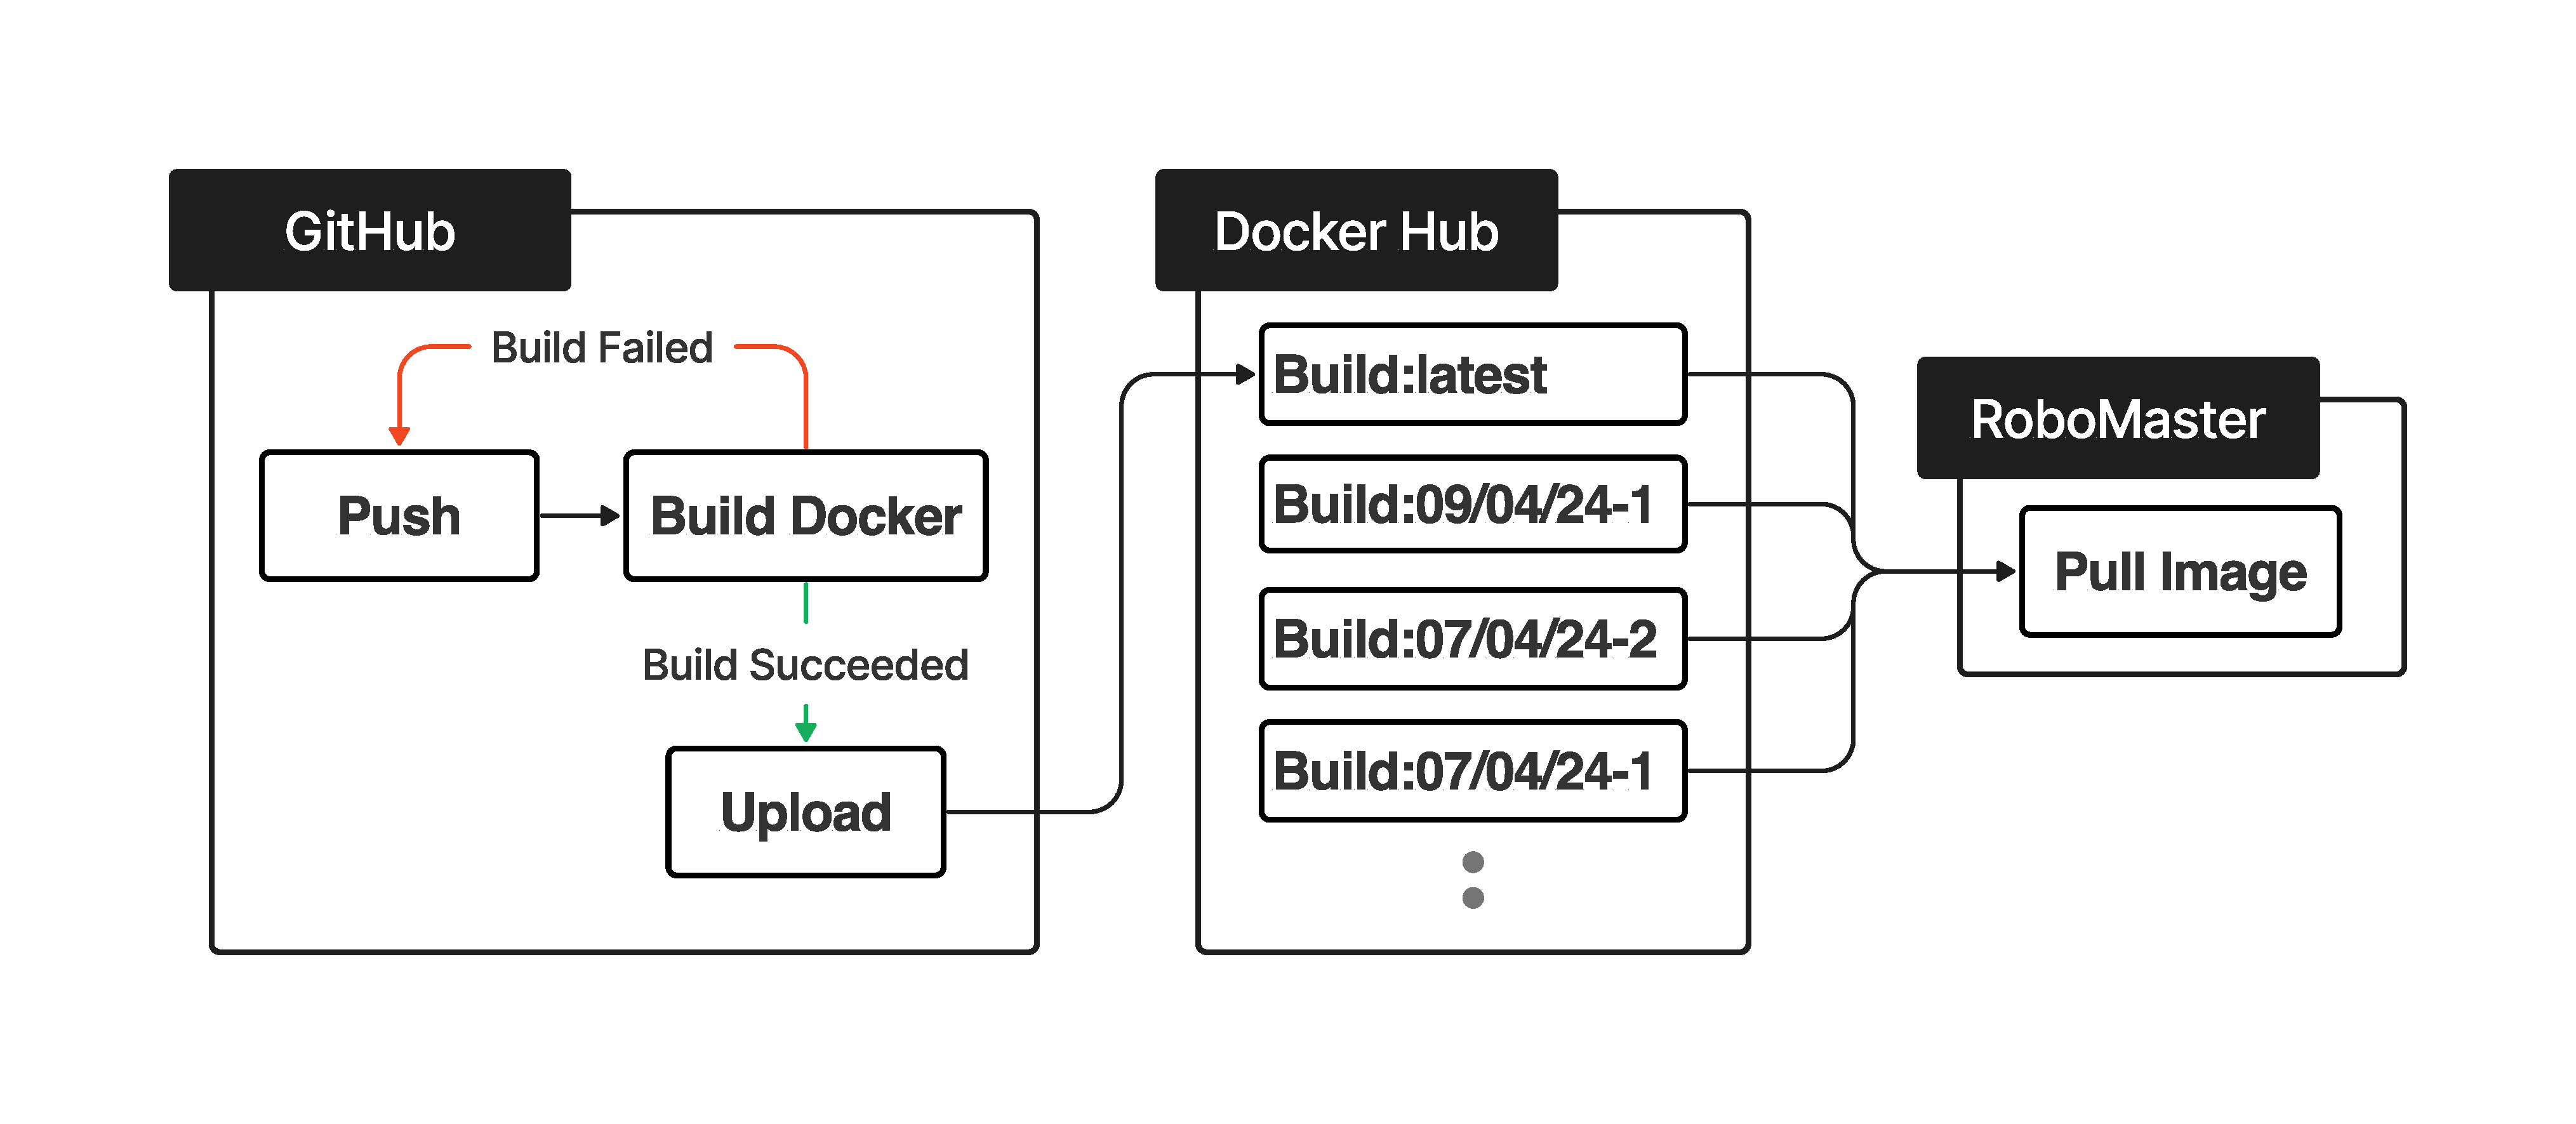
\includegraphics[trim=5cm 5cm 5cm 5cm, scale=0.2]{figures/cicd_diagram.pdf}

    \caption{Automated continuous integration pipeline for the Cambridge RoboMasters. Continuous deployment is implemented for the Raspberry Pi video publishers by pulling from Docker Hub and running the container on startup.}
    \label{fig:cicd-diagram}
\end{figure}


\section{Datasets}
\label{sec:datasets}
A variety of industry-standard datasets were utilized to benchmark the performance of my SLAM system, including the EuRoC Machine Hall \autocite{burri2016euroc} and TUM-VI \autocite{8593419} datasets. While these datasets provide a variety of sensors, we only utilize a monocular video as input when evaluating performance. Further information about each dataset is provided in the \nameref{sec:benchmarking} section.

In addition to standard datasets, I also used the aforementioned custom datasets generated in the simulator simulated environment to use for testing.


